\documentclass[class=report, crop=false, 12pt,a4paper]{standalone}
\usepackage{enumitem}
\usepackage{float}
\usepackage[normalem]{ulem}
\usepackage{graphicx}
\usepackage{amsmath}
\usepackage{amssymb}
\usepackage{siunitx}
\usepackage{commath}
\usepackage{tikz}
\usetikzlibrary{positioning, fit, calc}   
\tikzset{block/.style={draw, thick, text width=3cm ,minimum height=1.3cm, align=center},   
line/.style={-latex}     
}  
\begin{document}
\section{Lift and drag}
Typical forces of interest for bodies in a flow are \textbf{drag} and \textbf{lift}. We can represent these in dimensionless form:
\begin{gather}
  \textrm{Drag coefficient: }c_D = \frac{F_D}{\frac{1}{2} \rho U_\infty^2S}\\
  \textrm{Lift coefficient: }c_L = \frac{F_L}{\frac{1}{2}\rho U_\infty^2S}
\end{gather}
Where $S$ is a representative area for the body, determined by convention.
\begin{figure}[H]
  \centering
  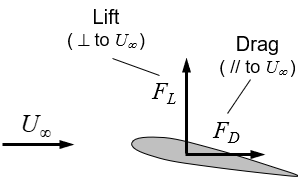
\includegraphics[width = 0.6\textwidth]{../img/diagram9.png}
\end{figure}
\section{Pressure and frictional force distribution}
\begin{figure}[H]
  \centering
  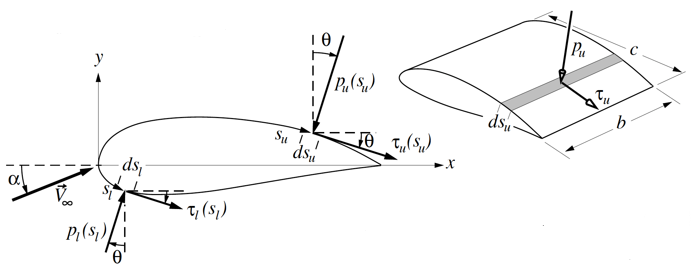
\includegraphics[width = 0.8\textwidth]{../img/diagram10.png}
\end{figure}
\begin{gather}
  L = - \int_{S}^{} \left( p (\hat{n}\cdot \hat{j}) \right)  \,\mathrm{d}S + \int_{}^{S} \left( \vec{\tau} \cdot \hat{j} \right)  \,\mathrm{d}S\\
  D = - \int_{}^{} \left(  p (\hat{n} \cdot \hat{j})\right)  \,\mathrm{d}S  + \int_{}^{} \left(\vec{\tau} \cdot \hat{i} \right)  \,\mathrm{d}S 
\end{gather}
To determine the lift and drag coefficients $c_L$ and $c_D$, we are interested in the pressure distribution over the airfoil, or more specifically in the local pressure difference from the stream pressure $p_{\infty}$.
\begin{equation}
  c_p = \frac{p - p_{\infty}}{\frac{1}{2} \rho V_{\infty}^2}
\end{equation}
Free stream pressure and velocity are $p_\infty$ and $V_\infty$.
\begin{figure}[H]
  \centering
  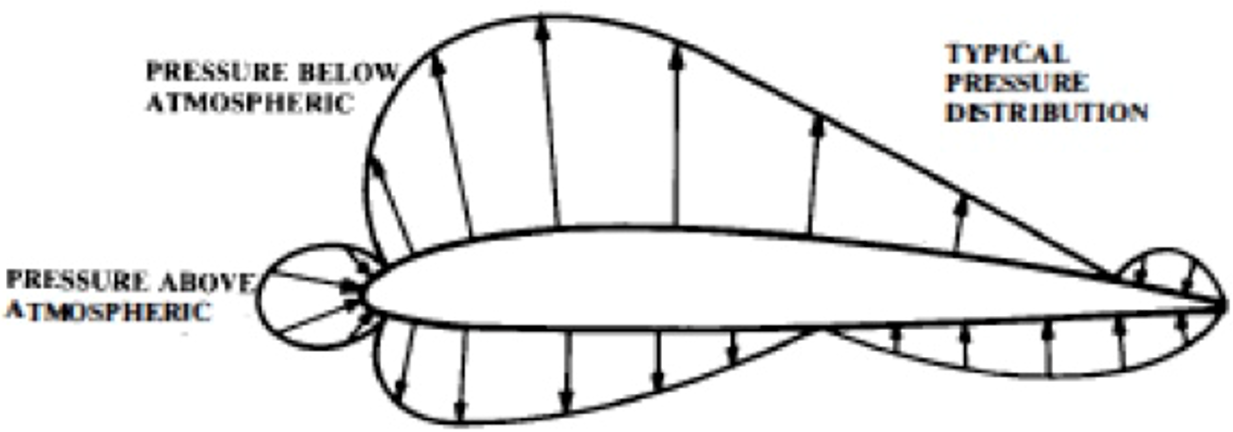
\includegraphics[width = 0.8\textwidth]{../img/diagram11.png}
\end{figure}
\begin{itemize}
  \item Local suction (depression): $c_p < 0$ Vectors point away from the airfoil surface
  \item Local pushing: $c_p > 0$ Vectors point towards the airfoil surface
\end{itemize}
\begin{figure}[H]
  \centering
  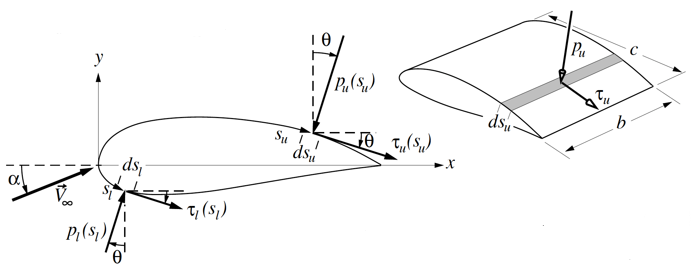
\includegraphics[width = 0.8\textwidth]{../img/diagram10.png}
\end{figure}
\begin{gather}
  L = - \int_{S}^{} \left(p\hat{n}\cdot \hat{j}\right)  \,\mathrm{d}S = \\
  c_L = - \frac{1}{S} \int_{S}^{} \left( \frac{p - p_{\infty}}{\frac{1}{2} \rho V_{\infty}^2} \hat{n} \cdot \hat{j} \right) \,\mathrm{d}S = -\frac{1}{S} \int_{S}^{} \left( c_p \hat{n} \cdot \hat{j} \right)  \,\mathrm{d}S  
\end{gather}
The lift coefficient per unit of span-wise length is:
\begin{equation}
  c_L' - \frac{1}{c}\int_{c}^{0} \left( c_p \hat{n}\cdot\hat{j} \right)  \,\mathrm{d}x 
\end{equation}
\section{Rearrangement of momentum equation - x direction}
\begin{gather}
  \rho \left( u \frac{\partial u}{\partial x} + v\frac{\partial u}{\partial y} \right) = -\frac{\partial p}{\partial x}  + \mu \left( \frac{\partial^2 u}{\partial x^2} + \frac{\partial^2 u}{\partial y^2} \right)\\
  \left(u \frac{\partial u}{\partial x} + v \frac{\partial u}{\partial y} \right) = \left(u \frac{\partial u}{\partial x} + v \frac{\partial u}{\partial y} \right) + v \frac{\partial u}{\partial y} - v \frac{\partial u}{\partial y}\\
  = - v \left(\frac{\partial v}{\partial x} - \frac{\partial u}{\partial y} \right) + \frac{1}{2} \left( \frac{\partial u^2}{\partial x} + \frac{\partial v^2}{\partial x} \right)\\
  = - v \left( \frac{\partial v}{\partial x} - \frac{\partial u}{\partial y} \right) + \frac{1}{2} \frac{\partial}{\partial x} (u^2 + v^2)
\end{gather}
$(u^2 + v^2)$ is the total kinetic energy of the fluid particle. The derivative is the element that takes into the account the variation of this kinetic energy. $\left( \frac{\partial v}{\partial x} - \frac{\partial u}{\partial y} \right)$ relates to the rotation of the particle. This rotation is related to the difference of velocity gradient.
\begin{gather}
  \rho \left[ -v \left( \frac{\partial v}{\partial x} - \frac{\partial u}{\partial y} \right) + \frac{1}{2} \frac{\partial}{\partial x} (u^2 + v^2) \right] = - \frac{\partial p}{\partial x} + \mu \left( \frac{\partial^2 u}{\partial x^2} + \frac{\partial^2 u}{\partial y^2} \right)\\
  - v \left( \frac{\partial v}{\partial x} - \frac{\partial u}{\partial y} \right) = - \frac{\partial}{\partial x} \left( \frac{p}{\rho} + \frac{u^2 + v^2}{2} \right) + \nu \left( \frac{\partial^2 u}{\partial x^2} + \frac{\partial^2 u}{\partial y^2} \right)   
\end{gather}
Our Bernoulli term in the above equation is $\left( \frac{p}{\rho} + \frac{u^2 + v^2}{2} \right)$, gravitational energy is negligible. $\left( \frac{\partial v}{\partial x} - \frac{\partial u}{\partial y} \right)$ is an anti-clockwise rotation. Hence, the vorticity component in the z direction is:
\begin{equation}
  \omega_z = \frac{\partial v}{\partial x} - \frac{\partial u}{\partial y}
\end{equation}
Our final momentum equations in $x$ and $y$ are: 
\begin{gather}
  -v \omega_z = - \frac{\partial}{\partial x} \left( \frac{p}{\rho} + \frac{u^2 + v^2}{2} \right) + \nu \left( \frac{\partial^2 u}{\partial x^2} + \frac{\partial^2 u}{\partial y^2} \right)\\
  u \omega_z = - \frac{\partial}{\partial y} \left( \frac{p}{\rho} + \frac{u^2 + v^2}{2} \right) + \nu \left( \frac{\partial^2 v}{\partial x^2} + \frac{\partial^2 v}{\partial y^2} \right)
\end{gather}
We can make some assumptions:
\begin{itemize}
  \item Inviscid flow - $\nu = 0$ (this may be realistic in some parts of a fluid domain but in real life, inviscid fluids do not exist)
  \item Irrotational flow - $\omega_z = 0$
\end{itemize}
This reduces our equations to:
\begin{gather}
  0 = - \frac{\partial}{\partial x} \left( \frac{p}{\rho} + \frac{u^2 + v^2}{2} \right) + 0\\
  0 = - \frac{\partial}{\partial y} \left( \frac{p}{\rho} + \frac{u^2 + v^2}{2} \right) + 0
\end{gather}
\section{Application of Bernoulli}
\begin{gather}
  p_\infty + \frac{1}{2} \rho V_\infty^2 = p + \frac{1}{2} \rho (u^2 + v^2) = \textrm{constant}\\
  c_p = \frac{p - p_{\infty}}{\frac{1}{2} \rho V_{\infty}^2} = 1 - \frac{u^2 + v^2}{V_\infty^2} = 1 - \frac{||V||^2}{V_\infty^2}
\end{gather}
\end{document}